\chapter*{Introduction}
\label{cap:introduction}
\addcontentsline{toc}{chapter}{Introduction}

In recent years...

\section{Motivation}


As mentioned in the introduction...

\section{Objectives}

The general objective of this project is...
\begin{enumerate}
	%\renewcommand{\theenumi}{\alph{enumi}}
	\item Search for animation datasets that are considered relevant for communicating with an \gls{npc} in a video game. These animations include dancing, greeting, pointing, sitting, fighting, and running.
	\item Automatic extraction of the aforementioned animations from animation banks and subsequent processing.
	\item Extraction of animations through motion capture from a heterogeneous group of users.
	\item Implementation, training, and comparison of different \gls{ai} models, including neural networks (LSTM, CNN, and RNN) as well as classical classification models (Random Forest).
	\item Development of a final application as a demonstration to showcase the results in \gls{vr} to enhance immersion.
\end{enumerate}

As a significant secondary objective, due to the lack of animation datasets, it has been proposed to publish the resulting datasets, both from artificial animations and user captures.

\section{Work Plan}


The work plan consists of several steps:

\begin{enumerate}
	%\renewcommand{\theenumi}{\alph{enumi}}
	\item Search for a dataset: generate a sufficiently large dataset with multiple examples of gestures to adequately train different models. This dataset should primarily consist of data from real users to identify the most natural gestures possible.
	\item Implementation of \gls{ai} models: implement various \gls{ai} models to compare them and determine which one is most suitable based on prediction speed and accuracy. The implementation of these models should include: training, a way to extract final model statistics, hyperparameter search, confusion matrix generator, and compatibility with a common user interface for all trainings.
	\item Development of a user interface for training and monitoring different models: develop a web interface so that users with less programming and \gls{ai} experience can train models capable of predicting the gestures they need without modifying the code or needing to understand the internal workings of the codebase.
	\item Development of a final application: create an application for Oculus Quest as a demo that connects to the chosen model and allows real-time usage demonstration.
\end{enumerate}

The development of tasks and their planning can be seen in Figure \ref{fig:diagrama-gantt-eng}.

\begin{figure}[H]
	\centering
	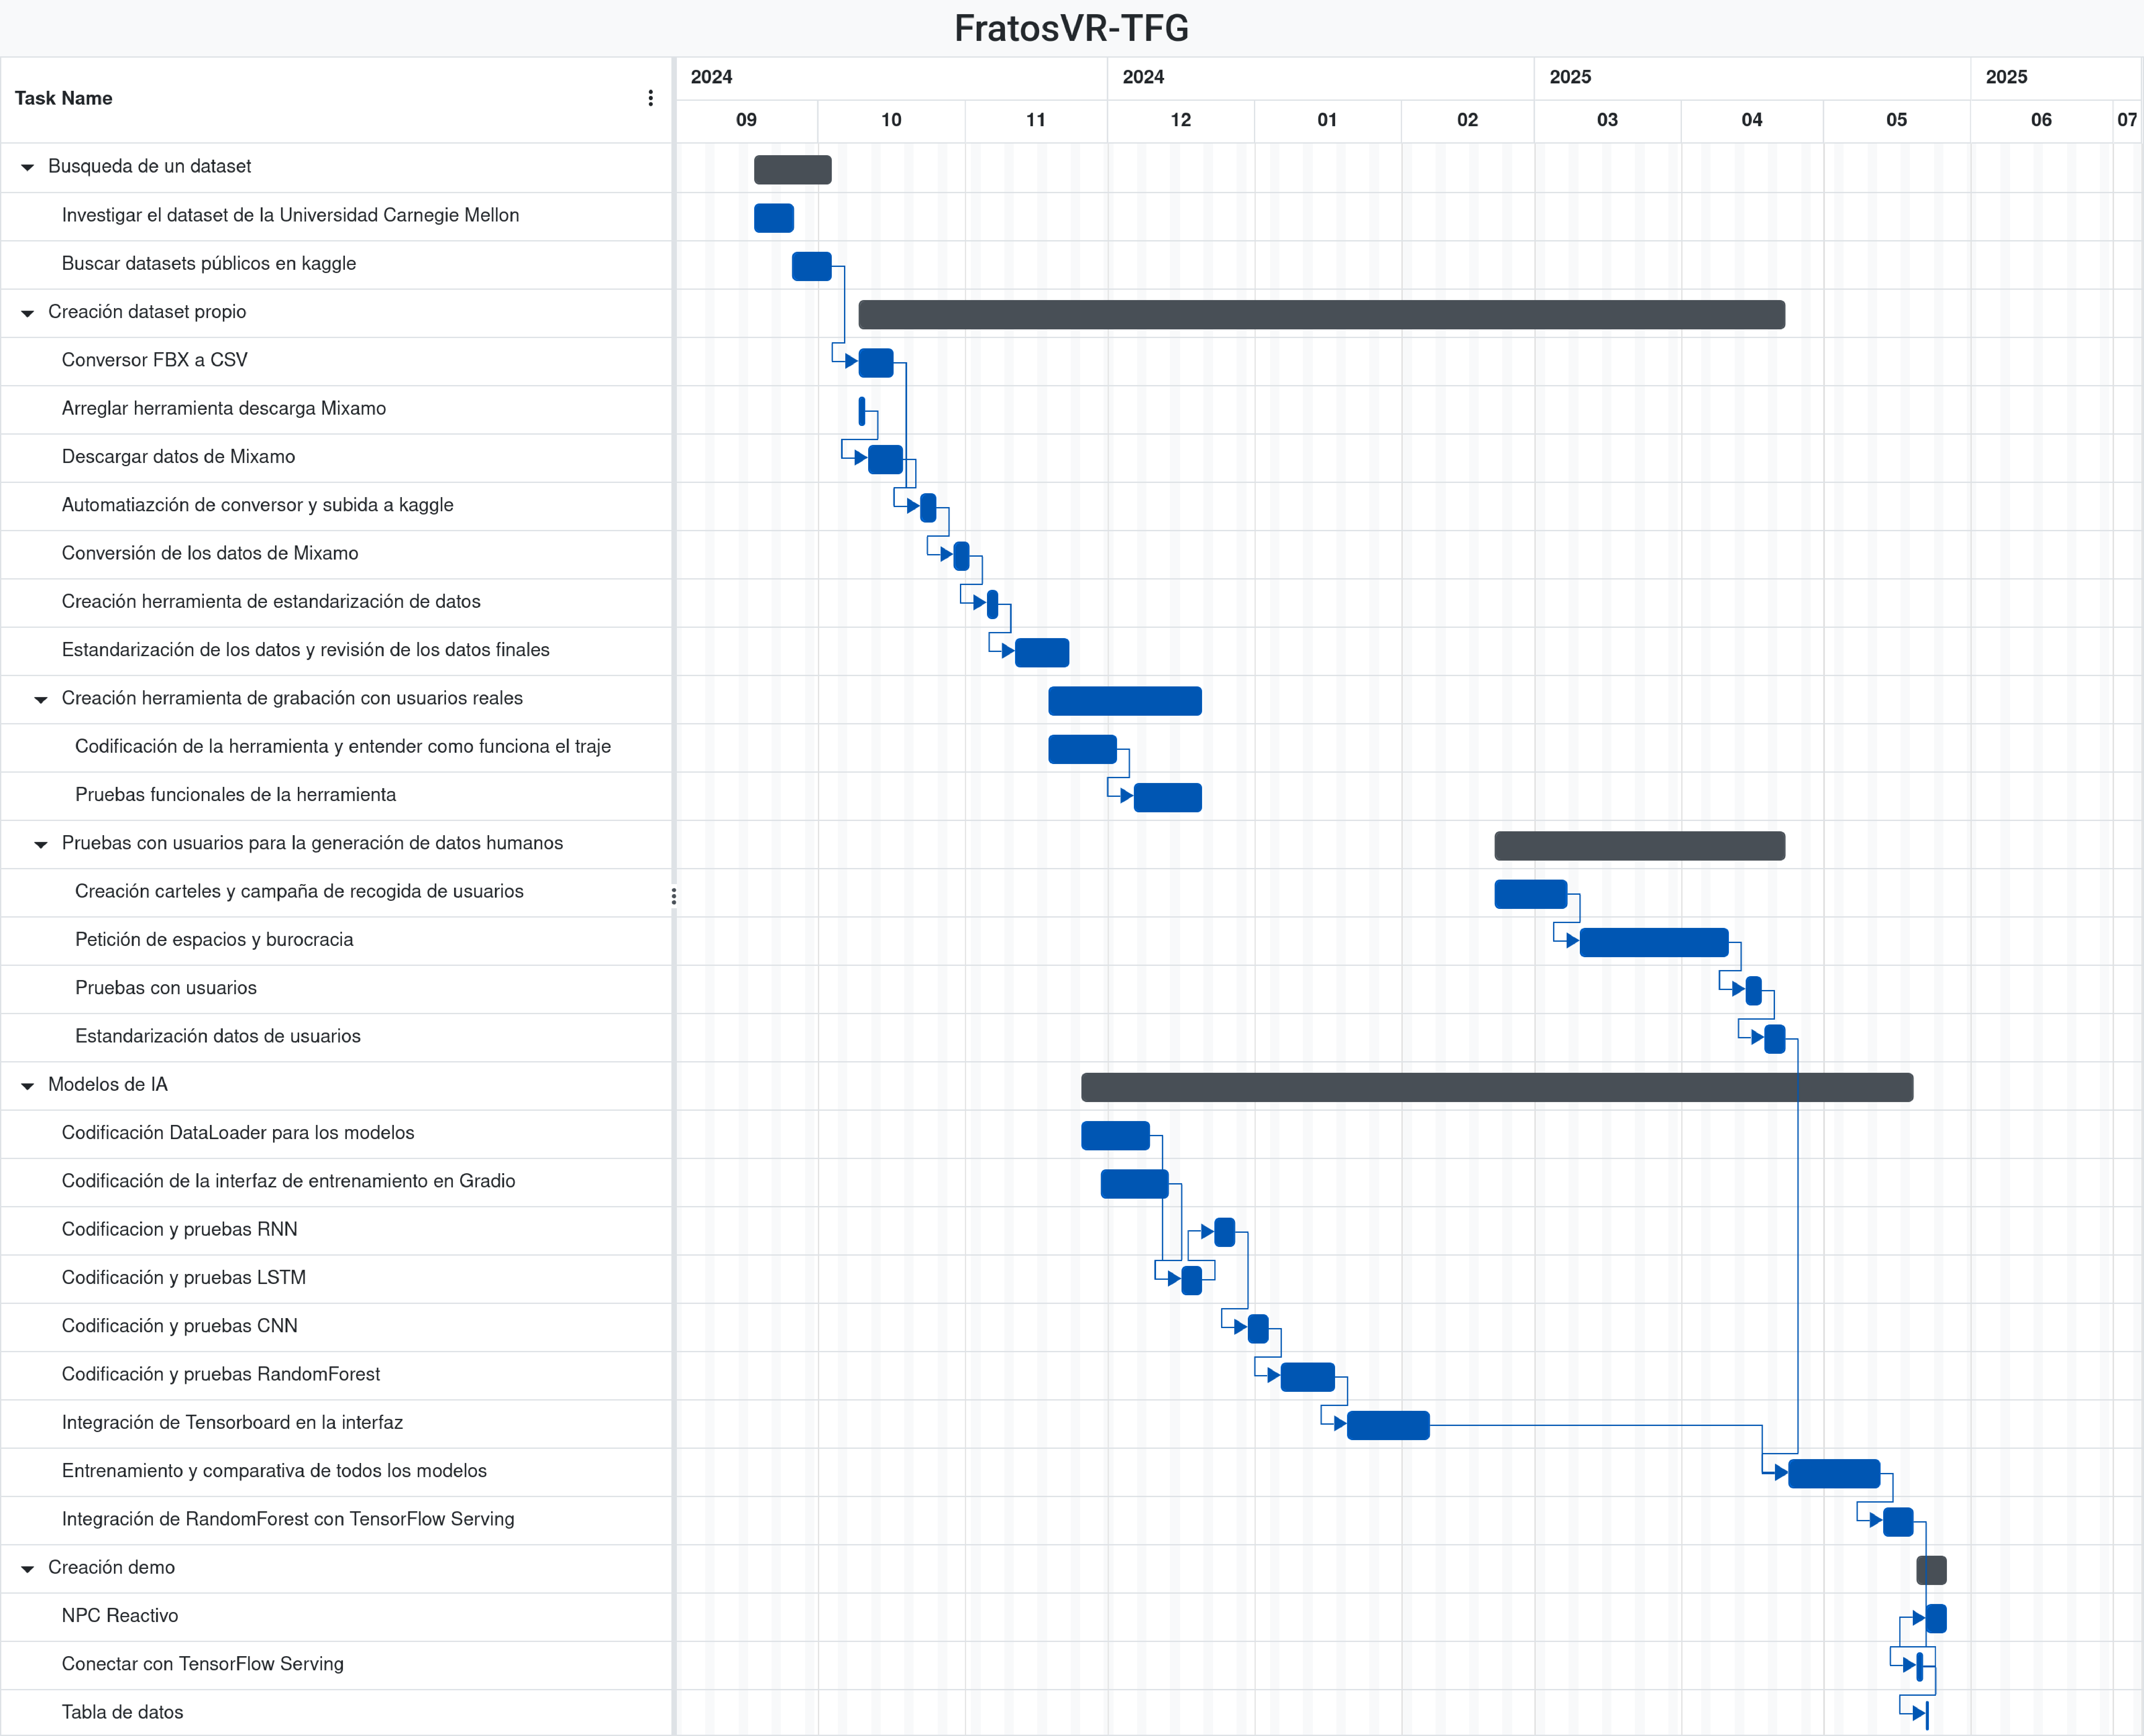
\includegraphics[width=0.91\textwidth]{Imagenes/Vectorial/Diagrama-gannt.pdf}
	\caption{Gantt chart of the project}
	\label{fig:diagrama-gantt-eng}
\end{figure}